
\begin{question}
Consider the following time series.

\begin{figure}
\centering
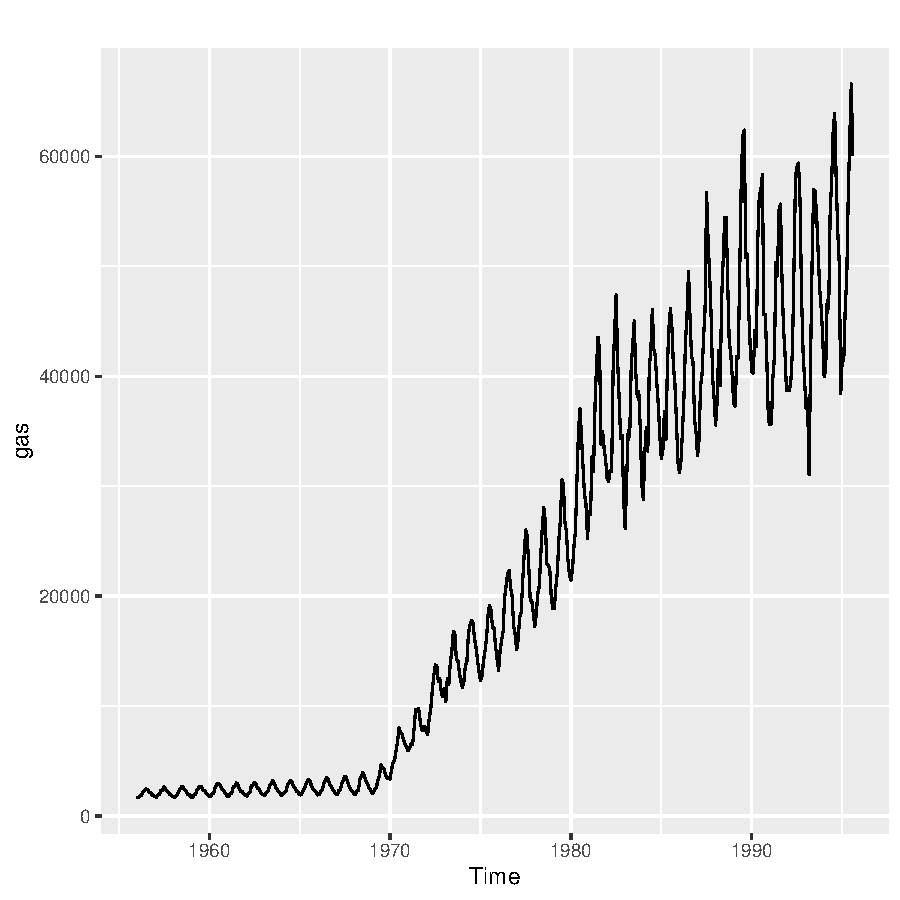
\includegraphics{unnamed-chunk-1-1.pdf}
\caption{plot of chunk unnamed-chunk-1}
\end{figure}

Which model is more appropriate to use?
\begin{answerlist}
  \item NA
  \item Use \(y_t = trend_t \cdot seas_t \cdot remainder_t\) * Use \(\ln y_t = \ln trend_t + \ln seas_t + \ln remainder_t\) * Use models with built in Box-Cox transformation * Use \(ETS(AAA)\)
  \item NA
  \item NA
\end{answerlist}
\end{question}

\begin{solution}
\begin{answerlist}
  \item False. Does not account for changing seasonality
  \item \begin{itemize}
\tightlist
\item
  True. * True. * True.
\end{itemize}
  \item NA
  \item NA
\end{answerlist}
\end{solution}

